\documentclass[a4paper,10pt]{article}
\usepackage[french]{babel}
\usepackage[utf8]{inputenc}
\usepackage[left=2.5cm,top=2cm,right=2.5cm,nohead,nofoot]{geometry}
\usepackage{url}
\usepackage{graphicx}
\usepackage{float}
\usepackage[colorinlistoftodos]{todonotes}
\usepackage{hyperref}

\linespread{1.1}



\begin{document}

\begin{titlepage}
\begin{center}
\textbf{\textsc{UNIVERSIT\'E DE MONTR\'EAL}}\\
%\textbf{\textsc{Faculté des Sciences}}\\
%\textbf{\textsc{Département d'Informatique}}
\vfill{}\vfill{}
\begin{center}{\Huge Rapport : TP1 - Sudoku}\end{center}{\Huge \par}
\begin{center}{\large Pierre Gérard, Alexandre Savard \\ 1121992-0957329}\end{center}{\Huge \par}
\vfill{}\vfill{} \vfill{}
\begin{center}{\large \textbf{IFT 3335 Intelligence artificielle: Introduction}}\hfill{\\Jian-Yun Nie, William Lechelle}\end{center}{\large\par}
\vfill{}\vfill{}\enlargethispage{3cm}
\textbf{Année académique 2015~-~2016}
\end{center}
\end{titlepage}

%\begin{abstract}
%Ce rapport présente ...
%\end{abstract}


\tableofcontents

\pagebreak


\section{Formulation du problème}
Nous cherchions à résoudre un sudoku à l'aide de trois algorithmes : la recherche, la recherche heuristique, et le hill climbing. 

Pour formuler ce problème comme un problème de recherche dans l'espace d'états, nous avons d'abord considéré la notion d'état comme étant une combinaison de chiffre à l'intérieur de la grille initiale. En d'autres termes, chaque fois que l'algorithme ajoute un chiffre à l'intérieur de la grille on se trouve dans un nouvel état. \\

Lorsque définie de cette façon, il est évident que l'état initial est la grille original contenant seulement les chiffres de départ. Dans notre cas, chaque noeuds correspond à la décision du chiffre à placer dans une case. Les noeuds enfants sont ainsi les grilles que nous aurions selon chaque chiffre possible. Par exemple si en observant la première case libre, l'algorithme avait le choix de mettre les chiffres 1, 5, 6, 8 et 9 dans la case sans créer de conflits, les 5 noeuds enfants serait la grille avec l'un des 5 chiffres précédents. \\

L'état but dans ce cas ci est l'état ou le sudoku est complètement remplit et qu'il ne contient aucune erreur. Nous vérifions que la grille est complète avec la fonction \verb|isFinished()|. Aussi, nous considérons que le coût d'une étape est égal à 1 pour la recherche simple et dépend de l'heuristique pour le hill climbing et la recherche avec heuristique.\\

Lorsque nous avons imposé une limite sur le nombre de noeuds visités à nos algorithme de recherche, il s'agissait donc d'imposer le nombre d'essais que l'algorithme pouvait faire. On parle d'un essai chaque fois que l'algorithme considère un chiffre à mettre dans une case, qu'il soit valide ou pas. 

\section{Search}
\subsection{Implémentation}
Cet algorithme a été implanté de façon à ce qu'il remplisse toujours la première case vide dans la grille. L'état initial est donc la grille vide qui doit être remplie et chacun de ses enfants sont les nouvelles grilles créés en mettant un chiffre de 1 à 9 dans la première case vide sans qu'il n'y ait de conflit. Par exemple, dans la première grille de la section \ref{sec:res} nous aurions A1 comme première case vide, et les possibilités de chiffres seraient 2, 4 et 5 puisque les autres chiffres créeraient des conflits. Les enfants de la première état dans l'arbre sera donc les 3 nouvelles grilles que l'on obtient à mettant un de ces 3 chiffres dans la première case vide. \\

Une fois que la première est remplie, il passe à la seconde case vide. Comme il s'agit d'un algorithme en profondeur d'abord, il va commencer par mettre le chiffre le plus petit qui n'a pas de conflit et passera directement à la prochaine case pour y mettre aussi le plus petit chiffre possible sans conflit. Si il se rend à une configuration impossible, il remonte de une étape et prend le second chiffre le plus élevé et ainsi de suite.\\

L'algorithme va s'arrêter seulement s'il réussit à remplir complètement la grille. Une fonction vérifie si la grille est exacte à la fin pour s'assurer du résultat. Cette algorithme peut aussi s'arrêter lorsque la limite de noeud visité est atteinte, il se solde alors par un échec.

\subsection{Résultat}
\label{sec:res}
Lorsque nous donnons une grille à cet algorithme, nous obtenons  d'abord la grille d'entrée pour bien visualiser le problème. Ensuite, si l'algorithme à réussit à remplir la grille avec le nombre d'essais permis, il nous affichera la nouvelle grille remplie. Par contre si la limite de noeuds est atteinte il affichera un message d'erreur. Voici un exemple:

\begin{verbatim}
   --- INPUT ---
. . 3 |. . . |6 . . |
9 . . |3 . 5 |. . . |
. . 1 |8 . 6 |4 . . |
---------------------
. . 8 |1 . 2 |9 . . |
7 . . |. . . |. . 8 |
. . 6 |7 . 8 |2 . . |
---------------------
. . 2 |6 . 9 |5 . . |
8 . . |. . 3 |. . 9 |
. . 5 |. 1 . |3 . . |
---------------------
\end{verbatim}

D'abord regardons le résultat si on donne une limite de 500 noeuds à l'algorithme:

\begin{verbatim}
--- Depth-First Search ---
ERROR : The limit number of node to be explored has been reached (500)
\end{verbatim}

Par contre si nous lui donnons une limite de 10000 noeuds, on obtient plutôt:

\begin{verbatim}
   --- Search ---
4 8 3 |9 2 1 |6 5 7 |
9 6 7 |3 4 5 |8 2 1 |
2 5 1 |8 7 6 |4 9 3 |
---------------------
5 4 8 |1 3 2 |9 7 6 |
7 2 9 |5 6 4 |1 3 8 |
1 3 6 |7 9 8 |2 4 5 |
---------------------
3 7 2 |6 8 9 |5 1 4 |
8 1 4 |2 5 3 |7 6 9 |
6 9 5 |4 1 7 |3 8 2 |
---------------------

Succes : Nombre de noeuds visites : 4999
\end{verbatim}

Ce qui est une solution optimale et par le fait même la seule solution valable à cette grille.


\subsection{Analyse des résultats}
Un tel algorithme devrait, en théorie, trouver chaque fois une solution au problème. Par contre, il devra parfois explorer une quantité phénoménale de noeuds avant d'y arriver. En considérant qu'il existe environ 5.5 millions de combinaisons possibles d'une grille de sudoku, il n'est pas surprenant que l'algorithme ne réussissent pas toujours lorsqu'on restreint son nombre d'essais à quelques centaines ou quelques milliers. En fait, il serait théoriquement possible que l'algorithme trouve une solution optimale en très peu d'étapes. Par exemple, avec une grille initiale contenant 27 chiffres de départs, il serait possible de résoudre cette grille en aussi peu que 54 essais, si on considère que l'algorithme trouve à chaque fois le bon chiffre à mettre dans la grille du premier coup. Mais cela n'est pas possible avec cette algorithme ci, car il n'est pas conscient de l'état global de la grille.  \\

Dans notre cas spécifique, nous avons donné une limite à l'algorithme pour pas qu'il ne travaille trop longtemps et pour voir la performance. En imposant une limite de seulement quelques centaines, les résultats étaient très mauvais. Par contre plus nous accordions une limite élevée, plus l'algorithme réussissait souvent à trouver une solution optimale. Ce qui est exactement ce à quoi nous nous attendions.

\section{Hill-climbing}

% Pierre
\subsection{Implémentation}
L'algorithme a été implémentée de manière à ce que la grille initiale soit remplie de manière totalement aléatoire. L'état initiale est donc cette grille initiale. On peut le visualiser comme la racine d'un arbre. Il a 9 enfants. Chaque enfant correspond a la permutation de (case1,case2) dans un des carré de dimension 3x3 telle que cette permutation minimise le nombre de conflit global. la permutation optimale est trouvé en les testant toutes à l'intérieur d'un carré 3x3\\

% condition d'arrêt

Cela permet d'affirmer que la probabilité que l'algorithme trouve une solution optimale tend vers 1 pour un très grand nombre d'essaie avec des configurations initiales différentes.

\subsection{Résultat}

Ci dessous un exemple de l'exécution du Hill-Climbing.
\begin{verbatim}
 --- INPUT ---
. . 3 |. 2 . |6 . . |
9 . . |3 . 5 |. . 1 |
. . 1 |8 . 6 |4 . . |
---------------------
. . 8 |1 . 2 |9 . . |
7 . . |. . . |. . 8 |
. . 6 |. . 8 |2 . . |
---------------------
. . 2 |. . 9 |5 . . |
8 . . |2 . 3 |. . 9 |
. . 5 |. 1 . |3 . . |
---------------------

-- Hill climbing --
4 8 3 |9 2 1 |6 7 5 |
9 6 7 |3 4 5 |8 2 1 |
2 5 1 |8 7 6 |4 9 3 |
---------------------
5 4 8 |1 6 2 |9 3 7 |
7 2 9 |5 3 4 |1 6 8 |
3 1 6 |7 9 8 |2 5 4 |
---------------------
1 3 2 |6 8 9 |5 4 6 |
8 7 4 |2 5 3 |7 1 9 |
6 9 5 |4 1 7 |3 8 2 |
---------------------
ECHEC, malgre 20 tests de configurations initiales differentes
Ci dessus, un maximum local (4 conflits restant)
\end{verbatim}
Comme indiqué, il reste 4 conflits et la solution proposé n'est pas une solution valide de sudoku, mais s'en approche.
Pour des grilles plus simple l'algorithme trouve bien la solution comme on peut voir ci-dessous.
\begin{verbatim}
	 --- INPUT ---
. . . |9 2 . |. 5 7 |
9 . 7 |. 4 5 |8 2 1 |
2 5 1 |8 7 6 |4 9 3 |
---------------------
5 4 8 |1 . 2 |9 7 6 |
7 2 9 |5 6 4 |1 3 8 |
1 3 . |7 9 8 |2 4 5 |
---------------------
3 7 2 |6 8 9 |5 1 4 |
8 1 4 |2 5 3 |7 6 9 |
. 9 5 |4 1 7 |3 8 2 |
---------------------

-- Hill climbing --
4 8 3 |9 2 1 |6 5 7 |
9 6 7 |3 4 5 |8 2 1 |
2 5 1 |8 7 6 |4 9 3 |
---------------------
5 4 8 |1 3 2 |9 7 6 |
7 2 9 |5 6 4 |1 3 8 |
1 3 6 |7 9 8 |2 4 5 |
---------------------
3 7 2 |6 8 9 |5 1 4 |
8 1 4 |2 5 3 |7 6 9 |
6 9 5 |4 1 7 |3 8 2 |
---------------------

Succes !
\end{verbatim}
Pour cette grille simple, Hill climbing a bien trouvé la solution optimale.
\subsection{Analyse des résultats}
Il n'est pas surprenant que Hill Climbing, un algorithme de recherche local, ne trouve pas de solution optimale. En effet, il est basé sur des changement locales et trouve régulièrement de bonne solution mais rarement la solution optimal. La figure suivante illustre cela.
\begin{figure}[H]
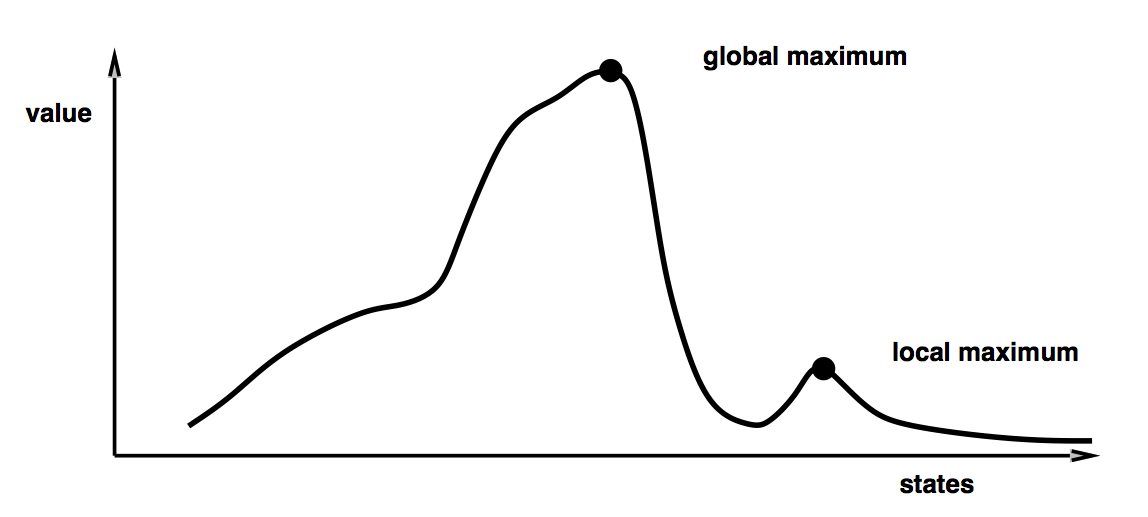
\includegraphics[scale=0.25]{images/hill-climbing.png}
\centering
\caption{Representation du maximum local}
\end{figure}
Une fois au maximum local, notre algorithme s'arrête comme il n'a pas de meilleur voisin. Il est incapable de dire si il existe un meilleur sommet puisqu'il est incapable de retourner en arrière pour modifier ces actions.\\

Une meilleur technique serait le "Simulated annealing", non demandé ici. Ceci permettrai à l'algorithme d'empirer son cas lorsqu'il est à un maximum pour éventuellement se retrouver sur un nouveau maximum, et ainsi de suite jusqu'à l'obtention du but.

 
\section{Heuristic search}

\subsection{Implémentation}

Pour réaliser une meilleur recherche une combinaison de 3 heuristique a été utilisé. Ces dernière sont les suivantes :\\ 

\begin{itemize}
	\item L'algorithme essaye de remplir d'abord les cases avec le moins de possibilités de chiffre différent.
\end{itemize}
Pour chacune des cases répondant a la condition ci-dessus, un cout de chemin est calculé qui dépendant des deux heuristique suivante :
\begin{itemize}
	\item La somme des possibilités restant dans les autres cases vides après avoir placé un chiffre à une case,
	\item L'inverse du nombre de case restant dans le carré, la ligne ou la colonne ou on place le chiffre.
\end{itemize}

Il semble évident que la première des heuristiques est la plus puissante des trois. Leur utilisation exclusive n'a pas beaucoup de sens. Elles ont donc été implémentée les 3 ensembles.

\subsection{Résultat}

Ci-dessous un exemple de différence entre l'algo sans et avec heuristique
\begin{verbatim}
--- Heuristic ---
4 8 3 |9 2 1 |6 5 7 |
9 6 7 |3 4 5 |8 2 1 |
2 5 1 |8 7 6 |4 9 3 |
---------------------
5 4 8 |1 3 2 |9 7 6 |
7 2 9 |5 6 4 |1 3 8 |
1 3 6 |7 9 8 |2 4 5 |
---------------------
3 9 2 |6 8 7 |5 1 4 |
8 1 4 |2 5 3 |7 6 9 |
6 7 5 |4 1 . |3 8 2 |
---------------------

Succes : Nombre de noeuds visites : 77



--- Depth-First Search ---
4 8 3 |9 2 1 |6 5 7 |
9 6 7 |3 4 5 |8 2 1 |
2 5 1 |8 7 6 |4 9 3 |
---------------------
5 4 8 |1 3 2 |9 7 6 |
7 2 9 |5 6 4 |1 3 8 |
1 3 6 |7 9 8 |2 4 5 |
---------------------
3 9 2 |6 8 7 |5 1 4 |
8 1 4 |2 5 3 |7 6 9 |
6 7 5 |4 1 9 |3 8 2 |
---------------------

Succes : Nombre de noeuds visites : 5313
\end{verbatim}
On remarque que le l'algorithme avec heuristique finit beaucoup plus rapidement. Le nombre de noeud visités a été diminué de 70 fois passant, pour cet exemple, de 5313 à 77.

\subsection{Analyse des résultats}

L'amélioration par rapport à une recherche classique sans heuristique est très importante. Le nombre de noeuds visités est de 77 au lieu de 5313 et cela pour un problème ou il n'existe pas toujours au moins une case avec une seule possibilité.\\

Pour les sudoku faciles, tel qu'il existe toujours au moins une case avec une possibilité, le nombre de noeuds visités serait égale au nombre de cases vides au départ.

% Pierre

\section{Comparaison}
Il est intéressant de comparer les résultats obtenus par nos trois algorithmes. D'abord le "Hill Climbing" n'à réussit absolument aucun sudoku de la liste de 100 que nous lui avons fournis en entré pour les raisons expliquées plus haut. On voit aussi que l'algorithme de recherche en profondeur d'abord peut prendre beaucoup plus d'essais avant de trouver une solution. En fait, si nous avions mis un nombre illimité d'essais avec des grille initiale différente, il aurait probablement performer près de la perfection, mais il aurait mis un temps très important à trouver une solution dans certain cas. En effet, il aurait fini par se retrouver dans un maximum local. Nous avons trouvé expérimentalement qu'il lui fallait 3000-4000 essais pour trouver un maximum global. Cependant, le hill climbing a l'avantage de trouver une solution (non-optimal) rapidement peu importe la difficulté de la grille.

Dans le cas le l'heuristique, il est évident qu'il est le meilleur des trois. Il arrive plus souvent à une solution puisqu'il visite beaucoup moins d'états avant d'arriver à une solution. Nous pouvons faire une comparaison visuelle les trois algorithmes dans le graphiques de la figure \ref{fig:comp} \\

\begin{figure}[H]
	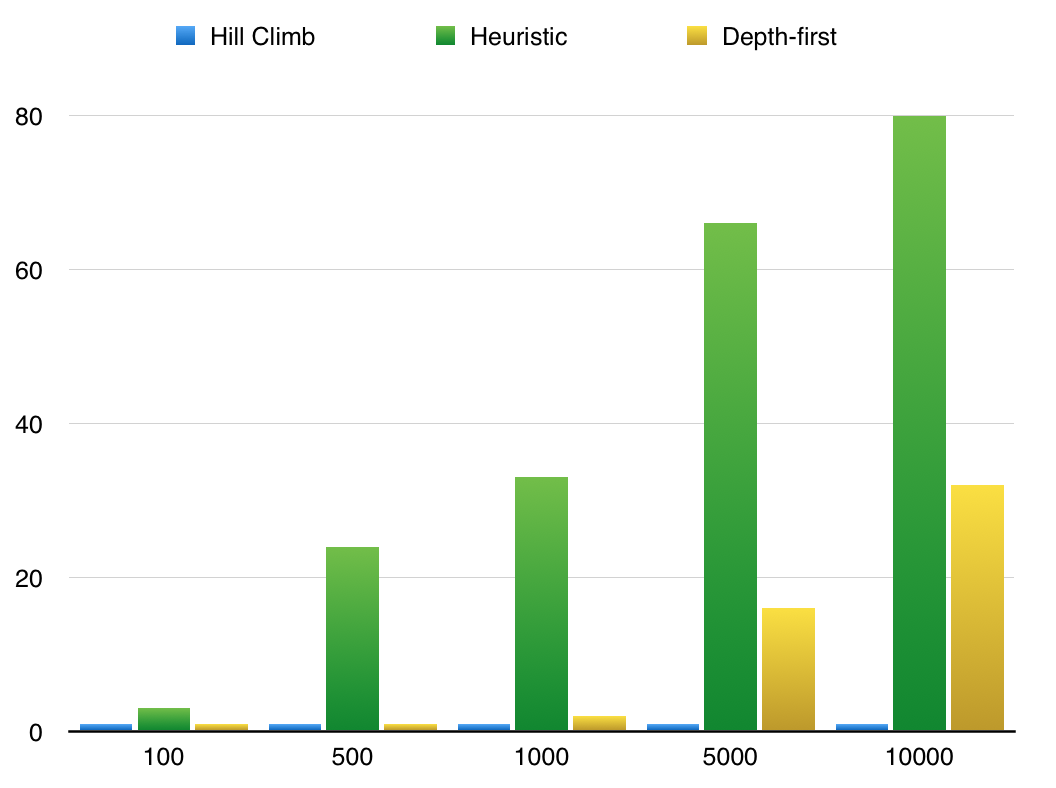
\includegraphics[width=12cm]{images/comparaison.png} 
	\centering
	\caption{Pourcentage de réussite pour les 3 algorithmes en fonction de la limite du nombre de noeuds}
	\label{fig:comp}
\end{figure}

On voit bien que pour 100 et 500 essais les algorithmes de "Hill Climbing" et de profondeur d'abord n'ont réussit aucun sudoku, par contre celui qui utilise notre heuristique à réussit, même avec très peu d'essais, à en résoudre quelques un. Plus on donne une grande quantité d'essais aux algorithmes plus il réussissent à trouver des solutions. Ceci est à l'exception du "Hill Climbing" qui échoue chaque fois puisqu'il reste pris dans un maximum local.\\

En comparant seulement les deux autres, on voit bien que l'algorithme qui utilise notre heuristique performe en général beaucoup mieux, mais plus on augmente la limite d'essais, plus la recherche en profondeur d'abord semble rattraper l'heuristique. Faute de puissance de calcul, nous n'avons pas pu tester plus de 10000 essais. 



\end{document}
